%%%%%%%%%%%%%%%%%%%%%%%%%%%%%%%%%%%%%%%%%%%%%%%%%%%%%%%%%%%%%%%%%%%%%%%%%%%%%%%
\chapter{Pesquisa em memória secundária}
%%%%%%%%%%%%%%%%%%%%%%%%%%%%%%%%%%%%%%%%%%%%%%%%%%%%%%%%%%%%%%%%%%%%%%%%%%%%%%%

Este capítulo aborda questões relacionadas a técnicas de armazenamento
e recuperação de dados em memória secundária.

%%%%%%%%%%%%%%%%%%%%%%%%%%%%%%%%%%%%%%%%%%%%%%%%%%%%%%%%%%%%%%%%%%%%%%%%%%%%%%%
\section{Memória secundária}
%%%%%%%%%%%%%%%%%%%%%%%%%%%%%%%%%%%%%%%%%%%%%%%%%%%%%%%%%%%%%%%%%%%%%%%%%%%%%%%

A classificação de dispositívos físicos pode ser feita ao considerar:
\begin{enumerate}
\item Desempenho no acesso aos dados.
\item Custo por unidade de dados.
\item Confiabilidade para casos de perda de dados em falhas de
energia ou falha do sistema, ou mesmo falha física do dispositívo.
\end{enumerate}
Também pode-se diferenciar armazenamento em:
\begin{description}
\item[Volátil] perde dados quando é desligado.
\item[Não-volátil] persistente mesmo quando é desligado. Inclui armazenamento
secundário e terciário.
\end{description}

%%%%%%%%%%%%%%%%%%%%%%%%%%%%%%%%%%%%%%%%%%%%%%%%%%%%%%%%%%%%%%%%%%%%%%%%%%%%%%%
\subsection{Mídias de armazenamento}

As médias de armazenamento disponíveis em geral são:
\begin{description}
\item[Cache] a mais rápida e custosa, volátil, e gerenciada pelo hardware
do processador.

\item[Memória principal] acesso rápido da ordem de 10 a 100 nanosegundos (1 nanosegundo = $10^{-9}$).
Em geral muito pequena (ou muito cara) para armazenar todos os dados de um banco de dados.
Hoje  em dia, em alguns casos, armazena todo o banco de dados (\emph{memcached}).
Ela é volátil, sendo que os dados são pedidos na falta de energia ou falha do sistema.

\item[Flash] dados sobrevivem em falhas de energia. Dados podem ser escritos em um local
uma única vez, porém podem ser escritos novamente.
Pode ser lida um número ilimitado de vezes, mas há um limite no  número de gravações
que varia entre 10K e 1M.
As leituras podem ser mais rápidas que a memória principal, mas as escritas
são lentas.
Muito usada em dispositivos embarcados como câmeras digitais, 
telefones, e memórias flash drive (pendrive).

\item[Magnética] dados são armazenados em uma mídia magnética com discos de movimento
giratório. 
Deve-se ler os dados do disco para a memória principal, e depois escrever de volta ao disco.
O acesso direto é possível em qualquer ordem, ao contrário de mídias de fita.


\item[Ótica] não volátil e os dados são lidos óticamente de um disco 
giratório através de um laser.
Os mais populares são CDROM (640 MB), DVD (4.7GB), e Blu-ray (27 GB a 54 GB).
As leituras e escritas são mais lentas comparadas a discos magnéticos.

\item[Fita magnética]
não volátil, usado primariamente para backup (recuperar falhas de disco), e 
arquivamento de dados.
O acesso é sequencial, muito mais lento que discos. Porém, a capacidade
de armazenamento é alta (40 a 300GB).
\end{description}

A figura~\ref{aula06:fig:media} ilustra a hierarquia de armazenamento de acordo com 
o desempenho e custo.
Os níveis mais altos são mais custosos, porém mais rápidos.
No sentido contrário, o custo por bit reduz, mas o tempo de acesso aumenta.
%
\begin{figure}[!htb]
\centering
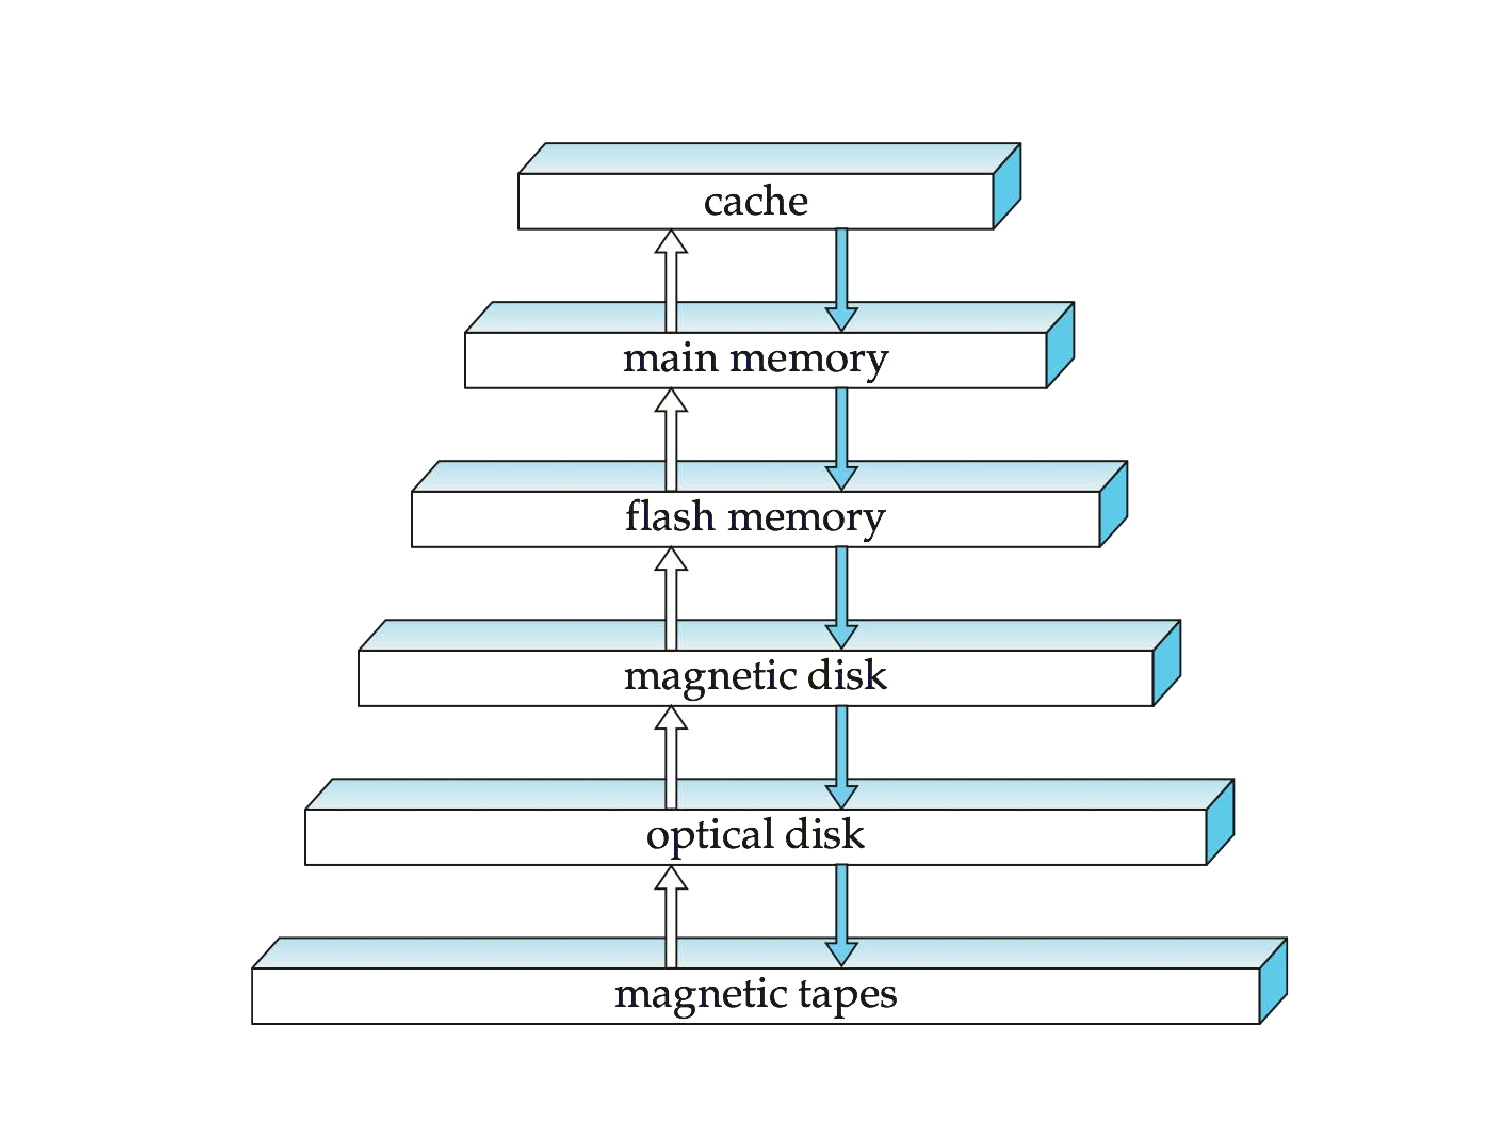
\includegraphics[width=0.6\textwidth]{aula06-media}
\caption{Hierarquia de mídias de armazenamento.}
\label{aula06:fig:media}
\end{figure}

Nessa hierarquia, podemos agrupar as mídias em:
\begin{description}
\item[Armazenamento primário] mais rápido mas volátil. Ex: cache, memória principal.

\item[Armazenamento segundário] próximo nível na hierarquia, não volátil,
acesso moderadamente rápido. Ex: memória flash, discos magnéticos.

\item[Armazenamento terciário] nível mais baixo, não volátil, tempo de acesso
lento. Também chamado armazenamento off-line. Ex: fita magnética, armazenamento ótico.
\end{description}

%%%%%%%%%%%%%%%%%%%%%%%%%%%%%%%%%%%%%%%%%%%%%%%%%%%%%%%%%%%%%%%%%%%%%%%%%%%%%%%
\subsection{Disco magnético}

\subsubsection{Estrutura física}

Fisicamente, discos magnéticos são simples.
A figura~\ref{aula06:fig:hd} mostra o funcionamento interno de um disco.
%
\begin{figure}[!htb]
\centering
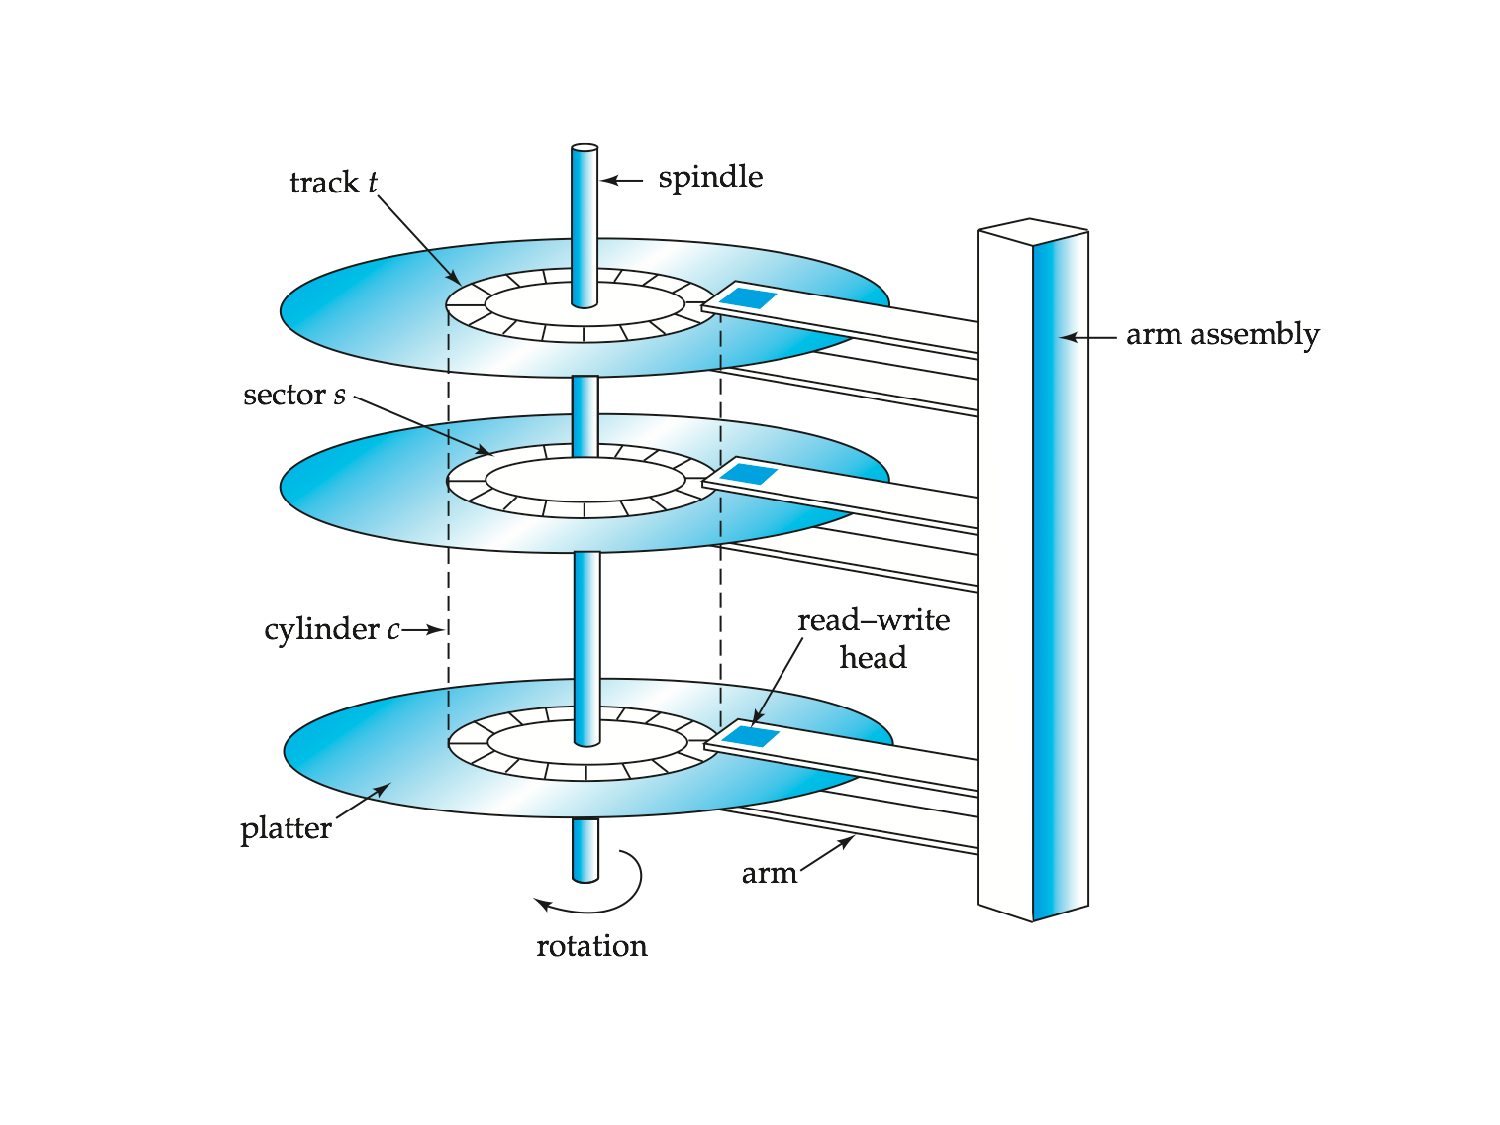
\includegraphics[width=0.6\textwidth]{aula06-hd}
\caption{Mecanismo de cabeças de leitura em um disco magnético.}
\label{aula06:fig:hd}
\end{figure}

Cada prato do disco tem duas superfícias com material magnético, onde a informação
é gravada.
O cabeçote de escrita-leitura (\emph{read-write head}) fica posicionada bem 
próxima a superfície do prato, e lê e escreve dados codificados magneticamente.
A superfície é dividida logicamente em {\bf trilhas}, que são subdivididas em 
\textbf{setores}. 
Um setor é a menor unidade que pode ser lida ou escrita do disco.
Em geral, um setor tem 512 bytes; há perto de 50K a 100K trilhas por prato, e 1
a 5 pratos por disco.

Os pratos são montados em braços de disco.
Para ler e escrever um setor, o braço do disco se move para posicionar o cabeçote
na trilha correta.
O prato gira, e os dados são lidos e/ou escritos a medida que o setor
passa pelo cabeçote.

Outro componente de discos é o {\bf controlador de disco} que faz a inteface 
entre o computador e o hardware do disco.
Ele aceita comandos de alto nível para ler e escrever setores.
Entre outras funções, garante checagem de erros.

\subsubsection{Medidas desempenho}

O \textbf{tempo de acesso} é o tempo que leva desde a solicitação de leitura/escrita
até o momento em que a transferência começa de fato. 
O tempo de acesso consiste em:
\begin{description}
\item[Tempo de busca] tempo que leva para reposicionar o braço na trilha correta.
O tempo médio de busca é 1/2 do pior tempo de busca, em geral 4 a 10 milisegundos.

\item[Latência rotacional] tempo que leva para o setor a ser acessado
aparecer debaixo do cabeçote. Latência média é 1/2 do pior caso, em geral
4 a 11 milisegundos em discos (5400 a 15000 rpm). 
\end{description}

A \textbf{taxa de transferência} é a taxa com que os dados são recuperados ou 
armazenados no disco. A taxa máxima é de 25 a 100 MB por segundo, e essa
taxa é menor para trilhas internas.

O \emph{Mean time to failure} (MTTF) é o tempo médio de funcionamento de um disco
sem falhas. 
Esse tempo varia entre 3 a 5 anos. 
A probabilidade de falhas em disco novos é baixa, que corresponde a um
``MTTF teórico'' de 500K a 1,2M horas.
Ou seja, um MTTF de 1,2M horas para um disco novo significa que dados 1000 novos discos,
na média um irá falhar a cada 1200 horas.

\subsubsection{Otimização de acessos}

A transferência de dados entre disco e memória ocorre em unidades de \textbf{blocos},
que são uma sequência continua de setores em uma única trilha.
O tamanho varia de 512 a vários kilobytes. Blocos pequenos podem implicar 
em várias transferencias do disco, enquanto que grandes blocos podem 
desperdiçar espaços devido a blocos parcialmente ocupados.
Um tamanho típico utilizado é de 4 a 16 kilobytes.

A otimização de acessos envolve \textbf{algoritmos de escalonamento} que são usados para ordenar o 
acesso às trilhas para minimizar o  movimento do braço.
O \textbf{algoritmo do elevador} funciona da seguinte forma:
\begin{enumerate}
\item move o braço do disco em uma direção (de dentro para fora ou de fora para dentro).
\item processa todas as requisições pendentes nessa direção.
\item reverte o movimento e repete a varredura.
\end{enumerate}

Outra forma de otimização é a \textbf{organização de arquivos} que otimiza o acesso ao
organizar os blocos, de modo a corresponder à forma com que os dados são acessados.
Exemplo é armazenar informações relacionadas em regiões próximas.
Arquivos podem se \textbf{fragmentar} com o passar do tempo.
Fragmentação acontece quando o arquivo é modificado, ou quando os blocos livres
estão espalhados, e novos arquivos tiverem que ocupar esses blocos.
O acesso sequencial a um arquivo fragmentado leva a maior movimentação do
braço do disco. 
Alguns sistemas possuem utilitários para \textbf{desfragmentar} o sistema
de arquivos, de modo a acelerar o acesso.

%%%%%%%%%%%%%%%%%%%%%%%%%%%%%%%%%%%%%%%%%%%%%%%%%%%%%%%%%%%%%%%%%%%%%%%%%%%%%%%
\section{Organização de arquivos}
%%%%%%%%%%%%%%%%%%%%%%%%%%%%%%%%%%%%%%%%%%%%%%%%%%%%%%%%%%%%%%%%%%%%%%%%%%%%%%%

A pesquisa em memória secundária normalmente está associada a \textbf{pesquisa 
em bancos de dados}.
O banco de dados é armazenado como uma coleção de arquivos. Cada arquivo
é uma sequência de registros, e cada registro é uma sequência de campos.

%%%%%%%%%%%%%%%%%%%%%%%%%%%%%%%%%%%%%%%%%%%%%%%%%%%%%%%%%%%%%%%%%%%%%%%%%%%%%%%
\subsection{Registros de tamanho fixo}

A estratégia mais simples é assumir \textbf{registros de tamanho fixo}.
Cada tabela possui o seu próprio arquivo, e cada arquivo possui registros
de um tipo específico de dado.
O cabeçalho possui informações de controle. Cada registro tem um ponteiro
especial, que aponta para o seu próximo registro.
O problema com essa abordagem é a ocupação parcial do bloco.
Por exemplo, cada registro ocupa 300 bytes e cada bloco ocupa 1024 bytes.
O cabeçalho ocupa 20 bytes. Qual o mínimo de espaço que será desperdiçado ?

Uma solução é permitir que registros cruzem a fronteira de um bloco. 
As alternativas para remoção do registro $i$ são:
\begin{enumerate}
\item mover registros $i+1$, ..., $n$ para $i$, ..., $n-1$.
\item mover registro $n$ para $i$.
\item não mover nada, ligar os registros vazios por uma \emph{free list}.
\end{enumerate}

Com \emph{free lists}, pode-se usar um ponteiro especial para guardar os registros livres.
Ela é uma representação mais eficiente que reusa o espaço destinado
aos atributos dos registros para guardar os ponteiros.
O cabeçalho possui informações de controle como ponteiro para o primeiro registro
com dados do bloco, e ponteiro para o primeiro registro livre do bloco.

O principal problema dessa abordagem é o desperdício de espaço dentro do bloco.

%%%%%%%%%%%%%%%%%%%%%%%%%%%%%%%%%%%%%%%%%%%%%%%%%%%%%%%%%%%%%%%%%%%%%%%%%%%%%%%
\subsection{Registros de tamanho variável}

A estrutura de \textbf{slotted-page} é comumente utilizada para organizar
registros de tamanho variável dentro de um bloco.
A figura~\ref{aula06:fig:slotted} ilustra a estrutura.
%
\begin{figure}[!htb]
\centering
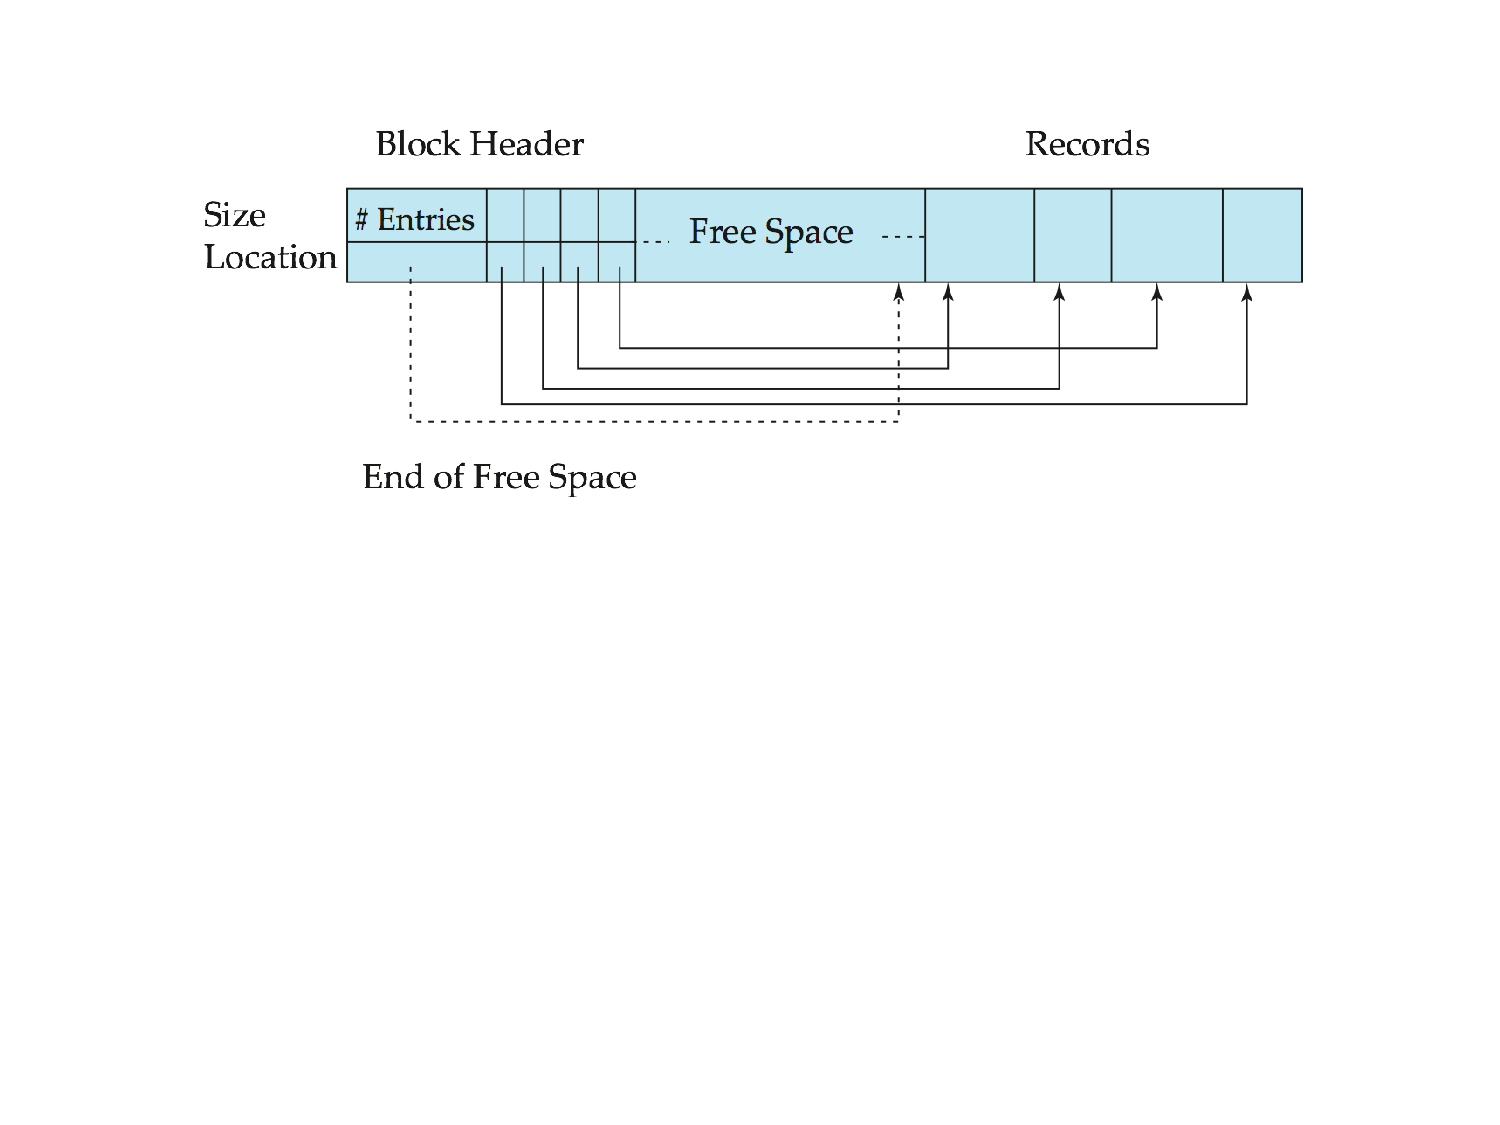
\includegraphics[width=0.8\textwidth]{aula06-slotted}
\caption{Estrutura do \emph{slotted-page}.}
\label{aula06:fig:slotted}
\end{figure}
O cabeçalho contém:
\begin{itemize}
\item número de registros.
\item localização e tamanho de cada registro.
\item fim do espaço livre no bloco.
\end{itemize}
Os registros podem ser movidos dentro de uma página para evitar espaços vazios
entre eles; as entradas no cabeçalho precisam ser atualizadas.
Ponteiros não apontam diretamente para o registro, mas apontam 
para o ponteiro de entrada do registro no cabeçalho.

Registros de tamanho variável aparecem em bancos de dados de diversas formas:
armazenameto de múltiplos tipos de conteúdo em um mesmo arquivo;
armazenamento de atributos que possem tamanho variável.

Se as slotted-pages são do tamanho de um bloco, o problema dos registros que cruzam é eliminado.
Isso limita o tamanho dos registros em um banco de dados, o que é o caso padrão.

%%%%%%%%%%%%%%%%%%%%%%%%%%%%%%%%%%%%%%%%%%%%%%%%%%%%%%%%%%%%%%%%%%%%%%%%%%%%%%%
\section{Organização de registros em arquivos}
%%%%%%%%%%%%%%%%%%%%%%%%%%%%%%%%%%%%%%%%%%%%%%%%%%%%%%%%%%%%%%%%%%%%%%%%%%%%%%%

Até agora, vimos como representar registros em uma estrutura de arquivo.
Há várias formas de organizar registros em arquivos:
\begin{description}
\item[Heap] um registro pode ser posicionado em qualquer lugar onde haja espaço.

\item[Sequencial] registros armazenados em ordem sequencial, com base
no valor da chave de busca de cada registro.

\item[Hashing] um função hash calculada com base em alguns atributos do 
registro. O resultado especifica em que bloco do arquivo do registro
deve ser posicionado.
\end{description}

%%%%%%%%%%%%%%%%%%%%%%%%%%%%%%%%%%%%%%%%%%%%%%%%%%%%%%%%%%%%%%%%%%%%%%%%%%%%%%%
\subsection{Organização de arquivos sequencial}

Adequada para aplicações que executam processamento sequencial sobre todo o arquivo.
Os registros do arquivo são ordenados por uma \textbf{chave de busca}.

A operação de remoção usa \emph{free lists} para registros de tamanho fixo.

A inserção localiza a posição onde o registro deve ser inserido e:
\begin{enumerate}
\item se houver espaço no bloco, insere no bloco.
\item se for o último registro, insere em um novo bloco.
\item se houver espaço em um bloco vizinho, distribuir. Caso contrário,
insere em um novo \textbf{bloco de estouro} (\emph{overflow block}).
\item de qualquer forma, as cadeias de ponteiros precisam ser atualizadas.
\end{enumerate}
O uso de blocos de estouro demanda a reorganização do arquivo de tempo em tempo
para restaurar a ordem sequencial.

%%%%%%%%%%%%%%%%%%%%%%%%%%%%%%%%%%%%%%%%%%%%%%%%%%%%%%%%%%%%%%%%%%%%%%%%%%%%%%%
\subsection{Clusterização multitable}

Os registros de cada tabela podem ser armazenados em arquivos separados.
Em uma \textbf{clusterização multitable}, registros de tabelas diferentes são armazenados no mesmo 
arquivo.
A principal motivação para armazenar registros relacionados no mesmo bloco é minimizar
a entrada e saída.
A figura~\ref{aula06:fig:clustering1} ilustra a organização de um arquivo com clusterização.
Esse arquivo armazena registros de uma ou mais relações em cada bloco.
Tal organização permite a leitura de registros que podem satisfazer uma união por meio de 
uma leitura de bloco.
%
\begin{figure}[!htb]
\centering
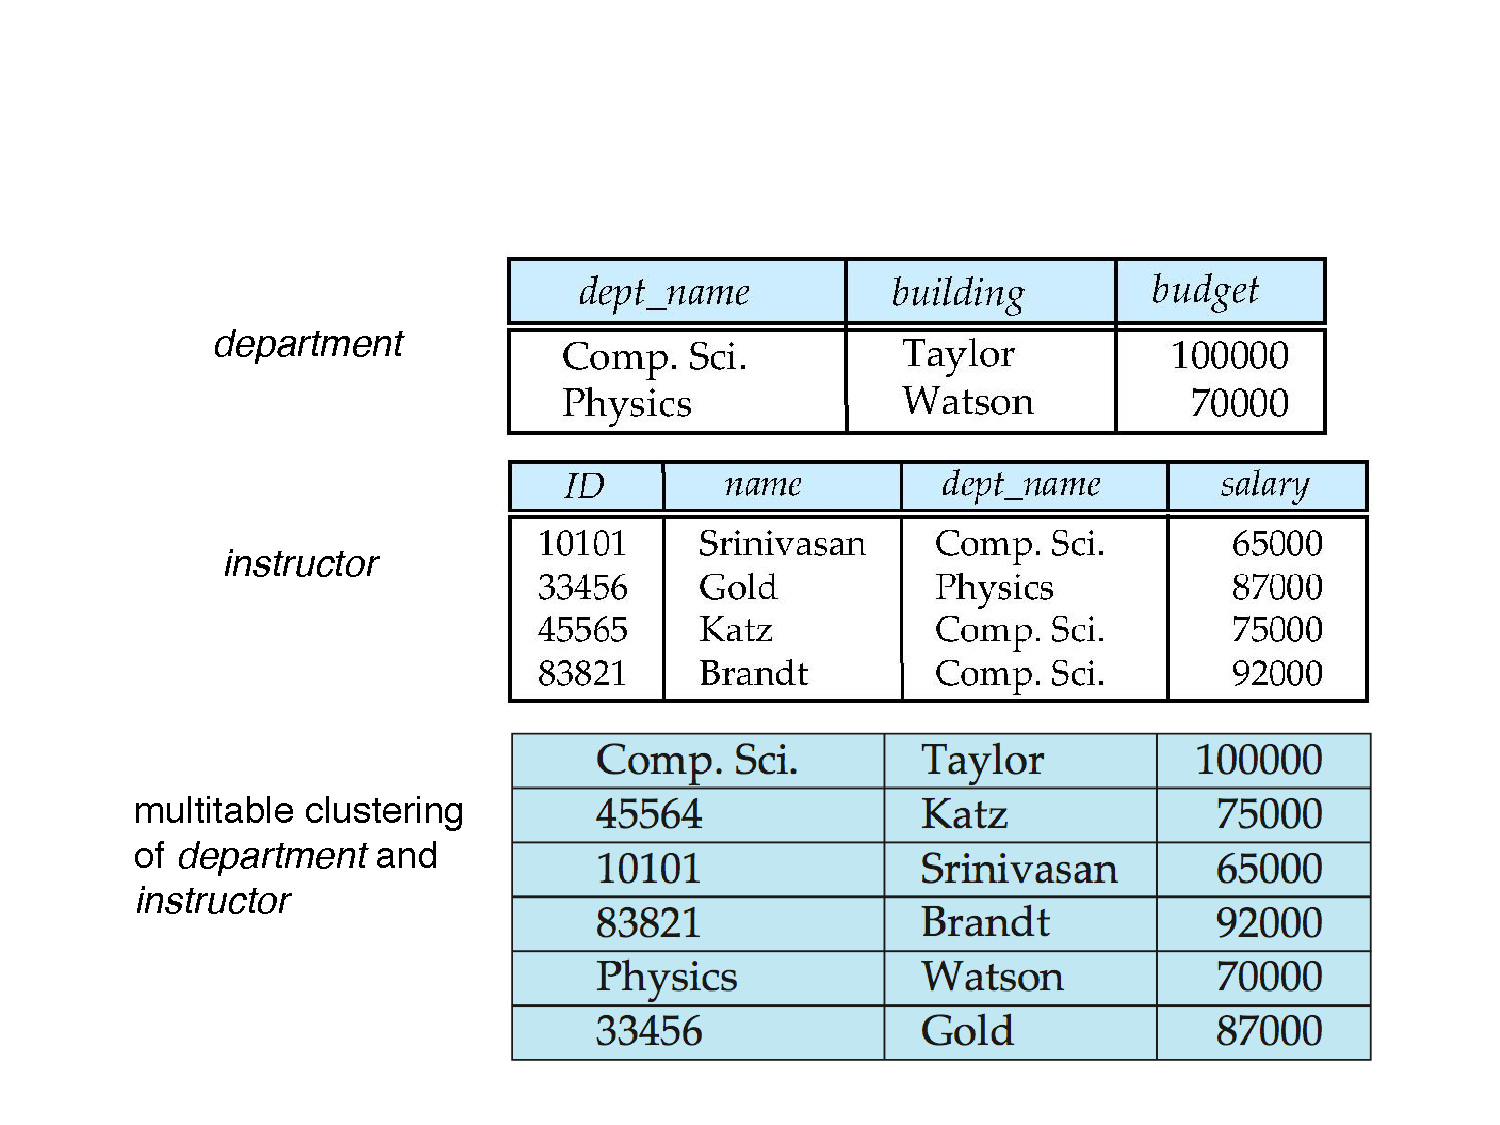
\includegraphics[width=0.6\textwidth]{aula06-clustering1}
\caption{Estrutura de arquivo de uma clusterização multitable.}
\label{aula06:fig:clustering1}
\end{figure}

Essa organização é boa para consultas com relação, e consultas envolvendo um único
deparamento e seus professores.
Porém, ela é ruim para consultas somente de departamentos.

%%%%%%%%%%%%%%%%%%%%%%%%%%%%%%%%%%%%%%%%%%%%%%%%%%%%%%%%%%%%%%%%%%%%%%%%%%%%%%%
\section{Sistemas de arquivos}
%%%%%%%%%%%%%%%%%%%%%%%%%%%%%%%%%%%%%%%%%%%%%%%%%%%%%%%%%%%%%%%%%%%%%%%%%%%%%%%

Em organizações de arquivos sequencias, cada tabela é armazenada em um arquivo.
O armazenamento poderia ser feito por meio do sistema de arquivos do sistema
operacional (SO).
A clusterização multitable pode trazer ganhos significativos em eficiência, mas 
essa organização não é compatível com o sistema de arquivos de sistemas operacionais.

Muitos dos sistemas de bancos de dados (SGBDs) de grande escala não utilizam diretamente o SO.
As tabelas são armazenadas em um único arquivo, e o SGBD gerencia o arquivos por conta própria.
Isso exige a implementação de um sistema de arquivos dentro do SGBD.

%%%%%%%%%%%%%%%%%%%%%%%%%%%%%%%%%%%%%%%%%%%%%%%%%%%%%%%%%%%%%%%%%%%%%%%%%%%%%%%
\subsection{Buffer manager}

O  número de transferencias de blocos entre o disco e a memória pode ser
reduzido mantendo o maior número possível de blocos na memória principal.
Um \textbf{buffer} é a porção da memória principal disponível para armazenar cópias
de blocos de disco.
O \textbf{buffer manager} é responsável pela alocação de espaço do buffer na 
memória principal.

Programas utilizam o buffer manager quando precisam ler um bloco do disco:
\begin{enumerate}
\item se o bloco já estiver no buffer, o gerenciador retorna o endereço 
do bloco na memória principal.

\item se o bloco não estiver no buffer, o manager:
	\begin{enumerate}
	\item aloca espaço no buffer para o bloco.
		\begin{enumerate}
		\item substituindo algum outro bloco, se necessário, para
			liberar espaço para o novo bloco.
		\item o bloco substituído é escrito de volta no disco somente se ele foi
		modificado desde a última vez que ele foi escrito/recuperado do disco.
		\end{enumerate}
	\item Lê o bloco do disco para o buffer e retorna o endereço do bloco
		na memóra principal para o programa.
	\end{enumerate}
\end{enumerate}

Sua função é similar ao gerenciamento e memória virtual dos sistemas operacionais.
Porém, bancos de dados tem requisitos diferentes.

%%%%%%%%%%%%%%%%%%%%%%%%%%%%%%%%%%%%%%%%%%%%%%%%%%%%%%%%%%%%%%%%%%%%%%%%%%%%%%%
\subsection{Políticas de substituição de blocos}

A maioria dos sistemas operacionais usam a política de substituição do bloco menos recentemente usado
ou \emph{least recently used} (LRU).
A ideia por trás do LRU é usar um padrão passado de referência a blocos como uma previsão de 
futuras referências, ja que usualmente nada mais se conhece.
Consultas possuem um padrão de acesso bem definido, com varreduras sequenciais.
O sistema do BD pode usar informação contida na consulta para prever referências futuras.

O LRU pode ser uma estratégia ruim para certos tipos de acesso que envolvem varreduras repetidas.
Por exemplo, na junção de 2 tabelas $r$ e $s$ por um laço aninhado. 
Uma estratégia mista é preferível, onde o otimizador de consultas pode oferecer dicas
para substituição de blocos.

Outras técnicas do buffer manager são:
\begin{description}
\item[Pinned block] bloco em memória que não tem permissão de ser escrito
de volta no disco.

\item[Estratégia Toss-immediate]  libera o espaço ocupado por um bloco assim que 
a última tupla do bloco é processada.

\item[Estratégia MRU] MRU significa mais recentemente usado (\emph{most recently used}), onde 
o sistema marca o bloco sendo processado. Depois que a última tupla do bloco é processada,
o bloco é desmarcado, e se torna o bloco mais recentemente usado.

\item[Saída forçada] o manager também suporta saída forçada de blocos para fins de 
recuperação.
\end{description}

%%%%%%%%%%%%%%%%%%%%%%%%%%%%%%%%%%%%%%%%%%%%%%%%%%%%%%%%%%%%%%%%%%%%%%%%%%%%%%%
\section{Índices densos e esparsos}
%%%%%%%%%%%%%%%%%%%%%%%%%%%%%%%%%%%%%%%%%%%%%%%%%%%%%%%%%%%%%%%%%%%%%%%%%%%%%%%

%%%%%%%%%%%%%%%%%%%%%%%%%%%%%%%%%%%%%%%%%%%%%%%%%%%%%%%%%%%%%%%%%%%%%%%%%%%%%%%
\section{Árvores de pesquisa}
%%%%%%%%%%%%%%%%%%%%%%%%%%%%%%%%%%%%%%%%%%%%%%%%%%%%%%%%%%%%%%%%%%%%%%%%%%%%%%%

%%%%%%%%%%%%%%%%%%%%%%%%%%%%%%%%%%%%%%%%%%%%%%%%%%%%%%%%%%%%%%%%%%%%%%%%%%%%%%%
\section{Índices Hash}
%%%%%%%%%%%%%%%%%%%%%%%%%%%%%%%%%%%%%%%%%%%%%%%%%%%%%%%%%%%%%%%%%%%%%%%%%%%%%%%

%%%%%%%%%%%%%%%%%%%%%%%%%%%%%%%%%%%%%%%%%%%%%%%%%%%%%%%%%%%%%%%%%%%%%%%%%%%%%%%
\section{Exercícios}
%%%%%%%%%%%%%%%%%%%%%%%%%%%%%%%%%%%%%%%%%%%%%%%%%%%%%%%%%%%%%%%%%%%%%%%%%%%%%%%

